\documentclass[12pt]{article}

% pacchetti 
\usepackage[italian]{babel}
\usepackage{graphicx}
\usepackage{svg}
\usepackage{url}

\usepackage{geometry}
 \geometry{
 a4paper,
 top=25mm,
 }
 
\usepackage{hyperref}
\hypersetup{
    colorlinks,
    citecolor=blue,
    filecolor=blue,
    linkcolor=blue,
    urlcolor=blue
}

\usepackage{amssymb}% http://ctan.org/pkg/amssymb
\usepackage{pifont}% http://ctan.org/pkg/pifont
\newcommand{\cmark}{\ding{51}}%
\newcommand{\xmark}{\ding{55}}%

%bibliography
\usepackage[sorting=none, isbn=false, eprint=false]{biblatex}
\addbibresource{bibliography.bib}


% set images path 
\graphicspath{ {./images/} }
% specify different fonts for headings 

\usepackage{color}

\definecolor{dkgreen}{rgb}{0,0.6,0}
\definecolor{mauve}{rgb}{0.58,0,0.82}
\definecolor{chromeyellow}{rgb}{1.0, 0.65, 0.0}

%______________Team's comments______________%

\newcommand{\edoardo}[1]{{\bf \color{red} Edoardo: #1 }}
\newcommand{\andrea}[1]{{\bf \color{mauve} Andrea: #1 }}
\newcommand{\davide}[1]{{\bf \color{chromeyellow} Davide: #1 }}
\newcommand{\piaget}[1]{{\bf \color{dkgreen} Piaget: #1 }}

%______________________Listing________________________%

\usepackage{listings}

\definecolor{codegreen}{rgb}{0,0.6,0}
\definecolor{codegray}{rgb}{0.5,0.5,0.5}
\definecolor{codepurple}{rgb}{0.58,0,0.82}
\definecolor{backcolour}{rgb}{0.95,0.95,0.92}

\lstdefinestyle{mystyle}{
    language=Java,
    aboveskip=5mm,
    belowskip=5mm,
    columns=flexible,
    backgroundcolor=\color{backcolour},   
    commentstyle=\color{codegreen},
    keywordstyle=\color{magenta},
    numberstyle=\tiny\color{codegray},
    stringstyle=\color{codepurple},
    basicstyle=\ttfamily\footnotesize,
    breakatwhitespace=false,         
    breaklines=true,                 
    captionpos=t,                    
    keepspaces=true,                 
    numbers=left,                    
    numbersep=5pt,                  
    showspaces=false,                
    showstringspaces=false,
    showtabs=false,                  
    tabsize=2
}

\lstset{style=mystyle}




\begin{document}
% pagina iniziale

\begin{figure}
    \centering
    
\includegraphics[width=0.2\linewidth]{images/unito_logo.jpg}
\end{figure}

\begin{center}
    \vspace{5ex}
    {\huge \textbf{Esame di Design Patterns}}
    \vspace{5ex}
\end{center}

\begin{center}
    Andrea Balbo Mossetto \\
    Davide Marietti \\
    Piaget Bouaka \\
    Edoardo Pastori
\end{center}

\vspace{10ex}

\begin{center}

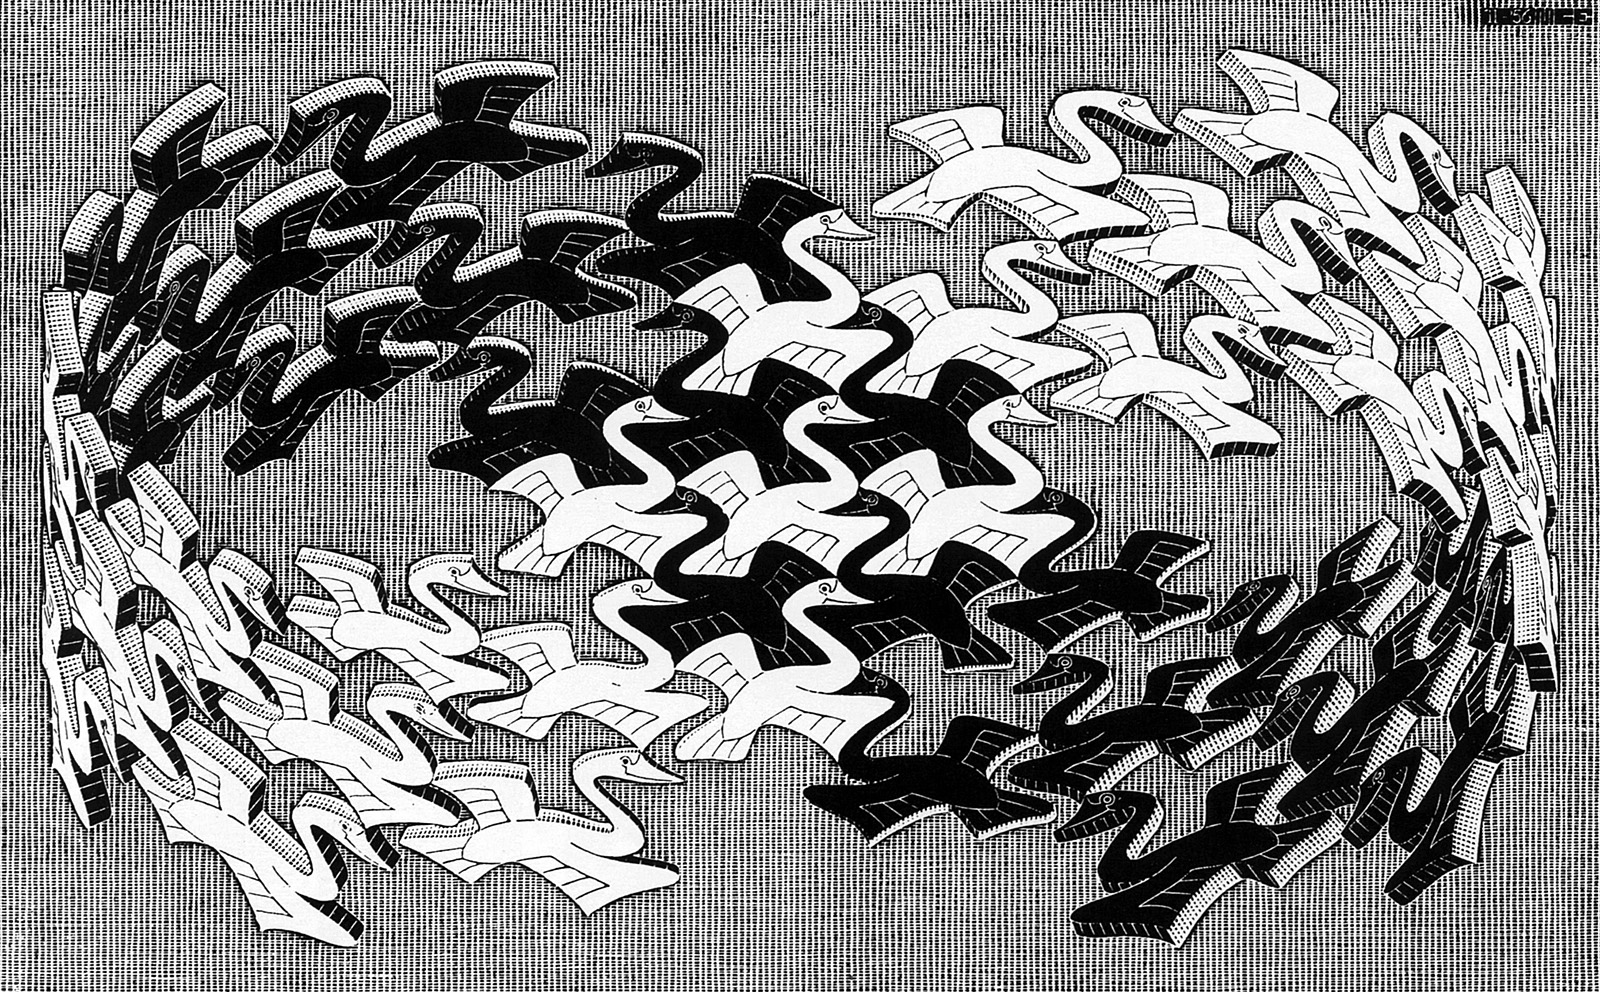
\includegraphics[scale=2]{design_pattern.jpeg}

\vspace{20ex}

Master IT Full Stack Design and Development, a.a. 2022/2023

\end{center}


\newpage

\tableofcontents

%\newpage
%\listoffigures

\newpage

\abstract{}
In questo documento \'e proposto il lavoro relativo alla realizzazione di un \textit{e-shop} di abbigliamento \textit{innovativo}. Una definizione pi\'u precisa di questo aggettivo ha richiesto una fase convergente, legata alla presa di coscienza delle caratteristiche proprie di quelli che sarebbero diventati i nostri \textit{competitors}, nonch\'e una fase divergente, attraverso la quale ci siamo soffermati sulle caratteristiche in linea con quella che iniziava a delinearsi con la nostra definizione di \textit{innovativo} mutuate da domini non appartenenti al mondo dell'\textit{e-shop} e dell'abbigliamento. 
\\
\davide{[TODO] Da AMPLIARE completandolo.}

\newpage

% capitoli 
\section{Elicitazione dei requisiti}
Questo capitolo raccoglie i requisiti che andranno poi analizzati, modellati e specificati nella fase di \textbf{Analisi dei Requisiti}. 
\\
\\
I problemi comuni da evitare in questa fase iniziale, per uno sviluppo florido del progetto, riferiscono a 3 domini principali:
\begin{enumerate}
	\item \textbf{Scopo}: i requisiti devono riflettere i bisogni del cliente
	\item \textbf{Comprensione}: \'e necessaria una buona comunicazione tra clienti, sviluppatori ed utenti per portare sul pratico i bisogni del cliente, che rifletteranno quelli degli utenti a cui vuole rivolgersi
	\item \textbf{Volatilit\'a}: i requisiti possono cambiare, non essere completi all'inizio dello sviluppo ed evolvere nel tempo; \'e quindi necessario definirli con quanta pi\'u perizia possibile in questa fase del processo
\end{enumerate}

\davide{\textbf{[TODO]} Ampliare la parte sugli strumenti utilizzati per fare la requirement elicitation.}

Si rende quindi necessaria una stretta comunicazione con il cliente, rappresentato dalla Professoressa Bono, per giungere ad un insieme di conoscenze che permetta di superare i problemi esposti poco sopra.

La strategia adottata \'e quella dell'\textbf{intervista}, alla quale siamo giunti dopo un \textit{brainstorming} che ci ha visto partecipi in un'iniziale definizione delle caratteristiche che, a nostro parere, dovrebbero appartenere ad un \textit{e-shop innovativo}.
Le nostre riflessioni sono sintetizzate nella sezione successiva. 


\subsection{Analisi di mercato e idee di prodotto} 

In questa fase abbiamo tratteggiato i contorni, ancora sfumati, dell'applicazione. Servono più informazioni possibili per avere una \textbf{visione ampia del mercato} in cui il prodotto richiesto si collocherà, ma anche idee originali a cui ispirarsi, che non devono necessariamente venire dal mondo dell'abbigliamento. Bisogna guardare al di là del {\em main stream}, l'applicazione dovrebbe creare l'effetto wow!

Un'analisi di mercato approfondita ci ha permesso di individuare e confrontare le caratteristiche dei competitors e di pensare a possibili \textbf{soluzioni innovative} non ancora presenti sul mercato da proporre al committente.

Le aziende di cui abbiamo analizzato i servizi offerti sono YOOX, Net a Porter, Patagonia, SSENSE e Garment Workshop.
Abbiamo innanzitutto preso in considerazione la possibilità di fare leva sulle capacità sartoriali del committente, per offrire vestiti su misura e la possibilità di mandarli in riparazione o ancora di effettuare un reso in cambio di voucher da poter utilizzare per nuovi acquisti. Ad eccezione della riparazione post vendita di Patagonia, nessuno di questi servizi è offerto dai competitors analizzati, come mostrato in tabella \ref{table:analisi_mercato_sartoria_interna}.

\begin{table}[h!]
\centering
\begin{tabular}{| c | c | c | c |} 
 \hline
  & Capi Su Misura & Riparazione Usato & Resi Per Voucher \rule[-2ex]{0pt}{6ex} \\
  \hline
 YOOX & × & × & × \rule[1ex]{0pt}{3ex}\\ 

 Net a Porter & × & × & × \rule[1ex]{0pt}{3ex}\\

 Patagonia & × & \checkmark & × \rule[1ex]{0pt}{3ex}\\

 SSENSE & × & × & × \rule[1ex]{0pt}{3ex}\\

 Garment Workshop & × & × & × \rule[-2ex]{0pt}{6ex}\\
 \hline
\end{tabular}
\caption{Tabella comparativa sulla capacità sartoriale.}
\label{table:analisi_mercato_sartoria_interna}
\end{table}

Superando gli aspetti non prettamente sartoriali, abbiamo notato un interesse da parte di ciascuno dei competitors ai temi etici e della sostenibilità, sebbene nessuno di questi abbia abbracciato definitivamente la causa, limitandosi solo ad alcuni (vedi il packaging) e tralasciandone altri (vedi l'economia circolare), come si può notare dalla tabella \ref{table:analisi_mercato}.

Risulta comune a tutti la presenza di una linea green nella propria offerta, ma considerando ad esempio il tema della sostenibilità ambientale, sociale e dell'economia circolare, solo Patagonia può dirsi promossa. Per quanto riguarda il tema della trasparenza finanziaria, solo Garment Workshop si distingue dagli altri.

Passando invece ad aspetti più legati alla tecnologia, si nota un utilizzo di algoritmi per la profilazione dei clienti online da parte della maggioranza delle aziende (mentre solo due utilizzano metodologie human driven).

Infine, è ancora abbastanza limitato l'utilizzo di strumenti innovativi, quali algoritmi di realtà aumentata che consentano di vedersi i vestiti digitali addosso dal proprio smartphone, l'invio di capi di abbigliamento senza che questi siano stati scelti dal cliente, o ancora l'abbandono del concetto di negozio fisso,  spostandosi ad un approccio più delocalizzato come gli spot stores di Garment Workshop.

\begin{table}[h!]
\centering
\begin{tabular}{|c |c | c | c | c | c | c | c | c | c | c | c | c|} 
 \hline
  & \parbox[t]{5mm}{{\rotatebox[origin=c]{90}{ Packaging }}} & \parbox[t]{5mm}{{\rotatebox[origin=c]{90}{ Sost. Ambientale }}} & \parbox[t]{5mm}{{\rotatebox[origin=c]{90}{ Sost. Sociale }}} & \parbox[t]{5mm}{{\rotatebox[origin=c]{90}{ Economia Circolare }}}  & 
  \parbox[t]{5mm}{{\rotatebox[origin=c]{90}{ Linea Green }}} &  \parbox[t]{5mm}{{\rotatebox[origin=c]{90}{ Test Di Invio Capi}}} & \parbox[t]{5mm}{{\rotatebox[origin=c]{90}{ Realtà Aumentata }}} &\parbox[t]{5mm}{{\rotatebox[origin=c]{90}{ Consigli Human Driven }}} &\parbox[t]{5mm}{{\rotatebox[origin=c]{90}{ Consigli Data Driven }}} &\parbox[t]{5mm}{{\rotatebox[origin=c]{90}{ Trasparenza Finanziaria }}} &\parbox[t]{5mm}{{\rotatebox[origin=c]{90}{ Spot Stores Temporanei }}}  \\
 \hline
 YOOX & \checkmark & × & × & × & \checkmark & × & × & × & \checkmark & × &  ×  \rule[1ex]{0pt}{3ex}\\ 

 Net a Porter & \checkmark & × & × & × & \checkmark & × & × & × & \checkmark & × &  ×  \rule[1ex]{0pt}{3ex}\\

 Patagonia & \checkmark & \checkmark & \checkmark & \checkmark & \checkmark & × & × & \checkmark & \checkmark & × &  × \rule[1ex]{0pt}{3ex}\\

 SSENSE & \checkmark & × & × & × & \checkmark & × & × & \checkmark & × & × &  ×  \rule[1ex]{0pt}{3ex}\\

 Garment Workshop & \checkmark & × & × & × & \checkmark & \checkmark & × & × & × & \checkmark &  \checkmark  \rule[1ex]{0pt}{3ex}\\[1.5ex]
 \hline
\end{tabular}
\caption{Tabella comparativa risultato dell'analisi di mercato.}
\label{table:analisi_mercato}
\end{table}

 

\subsection{Intervista}

L'intervista al committente dell'applicazione segue l'iniziale fase di analisi di mercato e di individualizzazione di possibili sviluppi innovativi, la quale è stata essenziale per \textbf{strutturare l'intervista} e raccogliere le idee innovative da proporre al committente. Le informazione raccolte nell'intervista serviranno a definire chiaramente i contorni dell'applicazione e a selezionare i moduli innovativi da sviluppare. L'intervista è stata strutturata nella seguente forma a macro blocchi:


\textbf{Chi:} in questa prima fase conoscitiva abbiamo voluto inquadrare meglio la figura del committente. Abbiamo chiesto:
\begin{itemize}
    \item {\em Descrizione dell'azienda. La sua dimensione e il fatturato? La localizzazione?} Il cliente è l'{\em Atelier Splendor}, una micro azienda di abbigliamento a gestione familiare, caratterizzata dalla presenza di una sartoria interna che produce vestiti con il proprio marchio. La sartoria comprende un unico punto vendita nel centro storico di Torino, con produzione nel retrobottega, dove, allo stato attuale, risultano impiegate solamente due sarte, le quali si occupano del loro ruolo in maniera tradizionale.
    Il cliente non ha specificato il proprio fatturato.
    \item {\em Chi sono gli utenti? Target utente finale è basso/medio/alto spendente? giovane/meno giovane, con quali valori e cultura)? Il target futuro deve rimane lo stesso?} Allo stato attuale, il target di clienti risulta alto spendente ed è concentrato nella fascia di età tra i 35 e i 60 anni. In generale il cliente dell'{\em Atelier Splendor} è colto e molto sensibile ai valori della sostenibilità. Emerge l'obiettivo futuro di ampliare il proprio target, estendendolo soprattutto in direzione di una fascia di età più giovane, comunque alto spendente, individuata più precisamente in neo assunti dai 25 anni in su.  
    \item {\em Su quale mercato opera attualmente? Su quale mercato punta di operare in futuro?} L'{\em Atelier Splendor} è attualmente presente come vendite sul solo mercato locale di passanti. Possiamo dunque identificare una clientela locale, prettamente circoscritta alla provincia di Torino. Dalle risposte del committente emerge la volontà di estendere il proprio bacino di clienti vendendo anche come negozio online, puntando con la giusta consapevolezza anche al mercato internazionale.
\end{itemize}

\textbf{Che cosa}: in questa seconda fase, sempre squisitamente conoscitiva, l'obiettivo è quello di comprendere nel dettaglio le esigenze del committente. Risulta a questo punto necessario carpire qual è la sua idea di applicazione finale e le caratteristiche salienti per lui imprescindibili. La raccolta di queste informazioni è stata essenziale per comprendere il contesto in cui si opera, al fine di selezionare le idee innovative (inizialmente pensate nella fase di analisi di mercato) più adatte da proporre al cliente.
\begin{itemize}
    \item {\em Cosa motiva lei e gli stakeholders? Quali sono i vostri valori? In particolare, quali le aspettative in merito al prodotto?} 
    Il cliente ha ribadito come durante questo processo di rapido sviluppo non voglia per nessun motivo allontanarsi dai suoi valori caratterizzanti: la cultura, la sostanza e la consapevolezza per se stessi e per l'ambiente. Il cliente dell'{\em Atelier Splendor} sceglie infatti un vestito per dire chi è, non lasciando decidere alla massa cosa dovrebbe indossare o chi dovrebbe essere. E' perciò emersa la tendenza al paradigma dello slow-fashion e della consapevolezza, contrapposta a strategie marketing di {\em hype} adoperate da altre aziende del mercato della moda ({\em e.g.} Supreme), rifiutando nettamente i canoni della GDO. L'azienda al centro di questo progetto desidera entrare nel mercato online seguendo il proprio stile e rispettando i propri valori fondanti.

    \item {\em Quali sono gli obiettivi dell’azienda? L’obiettivo principale, gli obiettivi a breve, medio e lungo termine (possibilmente in ordine di importanza)?} Il cliente è stato molto chiaro nella definizione dei propri obiettivi, ponendo come punto imprescindibile nel breve termine quello di avere un negozio online pienamente funzionante per espandere il proprio business. Guardando invece a un periodo più ampio, l'obiettivo principale è di farsi conoscere e apprezzare sulla scena internazionale della vendita online di abbigliamento, ritagliandosi una propria fetta di mercato che cresca nel tempo.

    \item {\em Quali sono i criteri di successo del prodotto? Quali potrebbero essere gli indicatori da monitorare durante il progetto e quale sarebbe un indicatore chiave per stabilire che l'applicazione ha avuto successo?}    
    Il cliente ha preferito non stabilire a priori un fatturato minimo da raggiungere o una quota di mercato da conquistare. Anche a causa della natura di realtà legata al territorio e alla volontà di sviluppo soprattutto come azienda, si è stabilito come indicatore chiave, cartina al tornasole del successo del progetto nella sua prima macro fase, l'impiego a tempo pieno con contratto a tempo indeterminato di nuovo personale nella sartoria, nello specifico di almeno due nuove sarte per il retrobottega.
\end{itemize}

\textbf{Quando}: in questa terza fase conoscitiva, puntiamo a definire con precisione le tempistiche relative alla finalizzazione del progetto. Lo scopo di queste domande è di carpire quali/quante idee innovative selezionare nella (successiva) fase di brainstorming con il committente. Il tempo a disposizione determina una selezione che andrà discussa con il cliente e una ripartizione delle idee di valore in moduli ``core", moduli ``pilota" e moduli non presi in considerazione in questa fase.
\begin{itemize}
    \item {\em Quando l'applicazione dovrebbe uscire sul mercato?}
    La scadenza per la pubblicazione online del sito di e-commerce è stata fissata a tre mesi dalla definizione dei dettagli definitivi da parte di tutti gli stakeholders. 
    \item {\em Quando l'applicazione dovrebbe essere pienamente operativa?}
    A seguito della pubblicazione, viene stabilito un tempo di due mesi per risolvere tutte le eventuali criticità e per sviluppare definitivamente tutti gli aspetti tecnici non essenziali, non presenti al momento del lancio.
    \item {\em Quando il progetto dovrebbe dirsi concluso?}
    La fine del progetto non è stata ancora definita, in quanto è stata lasciata aperta la possibilità di ulteriori fasi di sviluppo, che potranno essere prese in considerazione sulla base dei risultati raggiunti nel medio termine.
    
\end{itemize}



\textbf{Brainstorming}: in questa fase, sulla base di tutte le informazioni raccolte attraverso le precedenti domande durante l'intervista, abbiamo proposto al cliente tutte le nostre idee innovative relative a diversi possibili sviluppi del progetto. Le idee proposte sono state avvalorate da una precedente analisi di mercato e dalle conoscenze in merito del nostro esperto di dominio. L'insieme delle idee così raccolte, è poi stato ridiscusso con il cliente e suddiviso in gruppi, come presentato nella successiva sezione sui risultati.
\\

\subsection{Risultati}

I risultati dell'intervista possono essere suddivisi in tre macro gruppi.
Le idee che per motivi strategici o di tempo non vengono ulteriormente sviluppate sono finite nel gruppo dei moduli attualmente non presi in considerazione, e di seguito non presentati.

La progettazione e lo sviluppo completo dei \textbf{moduli ``core"}, strategici per raggiungere gli obiettivi del cliente e contribuire al tasso di innovazione dell'applicazione. L'investimento del cliente e le forze in gioco del team rendono questi obiettivi realistici e realizzabili.

\begin{itemize}
    \item {\em ``Pop-Up Stores"}: non molti negozi fisici, ma spot stores temporanei, localizzati dove sono concentrati la maggior parte dei clienti. La creazione di una rete di aziende amiche che condividono gli stessi ideali di sostenibilità permette numerosi vantaggi. {\em Atelier Splendor} ospiterà virtualmente i capi di queste aziende nel suo futuro negozio virtuale, queste aziende ospiteranno mostre temporanee dei nostri capi nei loro negozi fisici. La scelta delle città in cui organizzare le mostre verrà suggerita dai dati raccolti.
    \item {\em ``Vestirsi con la realtà aumentata"}: Algoritmo di realtà aumentata stile Ikea che consente di vestirsi virtualmente per provare i vestiti e trovare la propria taglia. Ciò sorride all'ambiente e fa l'occhiolino al consumatore consapevole perché permetterà di ridurre il numero dei resi. Cliente soddisfatto e ambiente pure. 
    \item {\em ``Magazzino Snello"}: rivedere il data model del magazzino da integrare in un data base pinco pallino su cui poggerà la nostra applicazione. Questo consentirà agli impiegati dell'azienda di loggarsi come tali e di monitorare meglio le risorse e i flussi di magazzino, abbattendo i costi generati dalla merce invenduta.
    \item {\em ``Go Circular!"}: sezione dell'applicazione dedicata ai vestiti usati che viene alimentata dai vestiti creati dall'atelier e dati indietro dai clienti in cambio di un vaucher da spendere sui vestiti nuovi confezionati dall'atelier. In questo modo il negozio ospiterà sì brand diversi e sostenibili, ma cerchiamo di favorire l'acquisto di abiti con il nostro brand. Questa politica, che sorride all'ambiente, sorride anche all'espansione della sartoria e all'assunzione di nuovo personale. Inoltre, gli abiti dati indietro spesso necessiteranno una sistemata da parte delle nostre sarte prima di essere caricato online.
    
\end{itemize}

La progettazione e lo sviluppo almeno parziale dei \textbf{moduli ``pilota"}, strategici ai fine del marketing e strategici in futuro, non appena verranno raggiunti gli obiettivi prefissati più importanti (assunzioni di nuove sarte e aumento del numero di clienti). Le condizioni attuali non consentono lo sviluppo completo di questi moduli. Lo sviluppo futuro di questi moduli consentirà una fruttuosa e duratura collaborazione con l'{\em Atelier Splendor}.
\begin{itemize}
    \item {\em ``Algoritmo di consiglio all'acquisto human-driven"}: l'output dell'algoritmo non viene direttamente fornito al cliente, ma è mediato dall'essere umano, nello specifico un esperto di moda, che spiega il perché di questo consiglio di acquisto.
    \item {\em ``Marketing"}: Nell'ambito del marketing, prodotti mirati saranno associati a un link di un contento TikTok di un influencer che starà indossando quel vestito. Questo per ampliare il target verso una fascia più giovane.
    \item {\em ``Sartoria dedicata e confezionamento su misura"}: la sartoria interna potrà essere ulteriormente allargata introducendo due nuovi servizi al cliente. Primo, i vestiti che necessiteranno di manutenzione (orli, pence, sostituzione cerniere, rattoppi, ...) potranno essere spediti alla sede centrale per essere aggiustati. Due, la sartoria offrirà la possibilità di avere abiti confezionati su misura.
\end{itemize}


\section{Analisi dei requisiti}

In questa sezione riportiamo i requisiti che la nostra applicazione dovrà rispettare e seguire nello sviluppo.

\davide{\textbf{[TODO]} Ampliare questa parte introduttiva.}

\subsection{Attori, obiettivi e Casi d'Uso}
\label{subsec:UC}

L'applicazione e tutto il sistema che traduce deve essere pensata per essere sfruttata da una serie di attori, umani o meno, che, con le loro attivit\'a, determinano come essa sar\'a sviluppata. Possiamo classificare gli attori nella tassonomia seguente:
\begin{itemize}
    \item Gli \textbf{attori principali} sono quelli che utilizzano direttamente l’applicazione per uno specifico use case (sono i fruitori dell’applicazione, e.g. un cliente, un impiegato).
    \item Gli \textbf{attori secondari} sono sistemi esterni (tipicamente software) che integriamo all’interno dell’applicazione (sono API che inseriamo per implementare il tutto e su cui non abbiamo controllo).
    \item Gli \textbf{attori fuori scena} sono entità che non usano direttamente l’app, ma che ne possono trarre benefici o ci danno dei vincoli da rispettare (l’università è l’attore fuori scena che beneficia di Moodle, la legge con il GDPR).
\end{itemize}

I Casi d'Uso, invece, descrivono i possibili scenari di utilizzo dell'applicazione, il macro-contesto all'interno del quale si muovono gli attori di cui sopra. Una comune rappresentazione grafica di un Caso d'Uso (od \textbf{UC}) \'e ravvisabile nell'{\em UC diagram}, ovvero un'\textit{interfaccia} astratta della nostra applicazione (cfr. fig. \ref{fig:UC_diagram}, p.\pageref{fig:UC_diagram}).
\\
\\
La definizione degli attori deriva da quella degli UC, pertanto ci aggiungiamo ad elencare quelli che saranno di nostro interesse progettuale:
\begin{itemize}
    \item Acquisto di capi di vestiario online (\textit{UC1}),
    \item Accesso al magazzino snello (\textit{UC2}),
    \item Aggiornamento dei clienti rispetto all'installazione temporanea di Pop-Up store (\textit{UC3}).
\end{itemize}

A questo punto possiamo enunciare gli attori, a pi\'u livelli, che entreranno in contatto con gli UC che abbiamo appena definito. In particolare:
\begin{itemize}
	\item \textbf{UC1}
		\begin{itemize}
		\item Principali: Cliente che vuole acquistare - Dipendente che monitora acquisti,
		\item Secondari: Metodi di pagamento,
		\item Fuori scena: Compagnia di trasporti .
		\end{itemize}
	\item \textbf{UC2}
		\begin{itemize}
		\item Principali: Cliente nella sua forma di avatar - Dipendente sarto che gestisce il proprio lavoro rispetto al traffico degli avatar,
		\item Secondari: Algoritmo che coadiuva i dipendenti nella gestione del magazzino,
		\item Fuori scena: Fornitori di materie prime.
		\end{itemize}
	\item \textbf{UC3}
		\begin{itemize}
		\item Principali: Cliente che vuole essere aggiornato rispetto alle attivit\'a della Compagnia, 
		\item Secondari: Database collegato a software tramite API per gestire informazioni di contatto dei clienti interessati alla newsletter,
		\item Fuori scena: GDPR.
		\end{itemize}
\end{itemize}

\subsection{Requisiti}

Con \textit{requisiti} intendiamo caratteristiche del sistema, da un punto di vista puramente logico o da un punto di vista tecnico. Pi\'u nello specifico, distinguiamo: 
\begin{itemize}
	\item \textbf{requisiti funzionali}, che riguardano ciò che il sistema fa e sono i moduli da implementare o integrare per lo sviluppo dell’applicazione,
	\item \textbf{requisiti non funzionali}, che riguardano come \'e fatto il sistema (riferendoci ad esempi quali i tools che vengono utilizzati per la sua realizzazione, il linguaggio di programmazione con cui \'e scritto, il database a cui si appoggia, ...).
\end{itemize}

Descriviamo quindi i requisiti che abbiamo intercettato relativamente agli UC individuati nella sezione precedente: 
\begin{itemize}
	\item UC1
		\begin{itemize}
		\item funzionali: voglio permettere all'utente di accedere al mio sito web e alla mia applicazione, visualizzare l'elenco degli articoli a mia disposizione, fargli scegliere quelli che pi\'u lo aggradano, inserirli nel carrello, pagare e completare l'ordine. Voglio permettere al dipendente di visualizzare gli ordini, 
		\item non funzionali: tools Java (pattern decorator + strategy), html + javascript + css (front-end), Oracle. 
		\end{itemize}
	\item UC2
		\begin{itemize}
		\item funzionali: voglio permettere all'utente di gestirsi (eventualmente) l'avatar, tramite cui provera' le diverse combinazioni di capi. I dati immagazzinati serviranno al sarto per una gestione pi\'u lean del magazzino (vedi anche ordini con i fornitori di materie prime),
		\item non funzionali: Oracle, Java (pattern Composite), Three-js (libreria js sul browser per realt\'a aumentata)/ webGL (grafica 3D).
		\end{itemize}
	\item UC3
		\begin{itemize}
		\item funzionali: voglio permettere ai miei "iscritti" di ricevere informazioni riguardanti i prossimi eventi pop-up store nella zona geografica di competenza,
		\item non funzionali: Oracle, Java (pattern Observer), client mail, API di geolocalizzazione.
		\end{itemize}
\end{itemize}

\vspace{0.5cm}
\begin{figure}[t]
  \centering
   \makebox[\textwidth][c]{\includesvg[width= 1.05\linewidth]{UC_diagram.svg}}
   \vspace{0.5cm}
  \caption{\small Esempio di UC diagram relativo all'applicazione del negozio online. All'interno delle {\em system boundaries} sono posizionati i casi d'uso esaminati in questa sezione. Gli attori principali (azzurro), quelli secondari (verde) e quelli fuori scena (giallo) sono rappresentati dalle figure al di fuori del {\em system} e sono collegati ai relativi casi d'uso. Una più approfondita analisi del diagramma è presentata in sezione \ref{subsec:UC}}
  \label{fig:UC_diagram}
\end{figure}


\subsection{Glossario degli attori}

Viene fornito al lettore un glossario dei termini tecnici utilizzati nelle sezioni precedenti:
\begin{itemize}
	\item API: \textit{``le API sono meccanismi che consentono a due componenti software di comunicare tra loro usando una serie di definizioni e protocolli. Ad esempio, il sistema software dell'ufficio meteorologico contiene dati meteorologici giornalieri. L'applicazione del meteo sul cellulare ``parla'' con questo sistema tramite API e mostra gli aggiornamenti meteorologici quotidiani sul telefono''} (cfr. \cite{bworld}).
	\item Client mail: un programma che permette di gestire il servizio di posta elettronica.
	\item Database: \textit{un database \'e una collezione organizzata e strutturata di dati. Il database \'e controllato da un Database Management System (DMBS), che funge da interfaccia tra l'utente che vuole avere accesso ai dati e il pc su cui questi dati sono salvati} (cfr. \cite{database}); un celebre esempio di DBMS e' Oracle. 
	\item Libreria: insieme di funzioni e strutture dati che permette allo sviluppatore di avere a propria disposizione codice gi\'a pronto alle proprie necessit\'a.
	\item Linguaggio di marcatura: insieme di regole che definiscono e strutturano l'impaginazione di un testo. Faremo in particolare ricorso ad \textit{HTML} e \textit{CSS}. La stesura di codice in questi linguaggi definir\'a ci\'o che gli utenti vedranno tramite interfaccia.
	\item Linguaggio di programmazione: linguaggio formale che specifica un insieme di istruzioni che vorranno interpretate e/o compilate dal computer, restituendo dei dati in uscita. Ci avvaliamo di \textit{Javascript} e \textit{Java}.
	\item Pattern (\textit{Design Pattern}): modello logico a cui si ricorre per proporre una soluzione ad un problema che riguarda l'architettura e la progettazione del programma. 
\end{itemize}


\section{Documento di vision}

\subsection{Visione}

Il progetto nasce dal desiderio di una piccola sartoria di Torino, fortemente legata al territorio, di investire a lungo termine sul proprio sviluppo commerciale.
\\
\\
L'azienda in questione esiste per soddisfare il bisogno di una clientela selezionata di vestire alla moda, con classe e stile. Possiede infatti il know-how necessario per la produzione di capi di alta qualità e per la riparazione sartoriale degli stessi. Risulta inoltre presente da anni sul mercato, di cui conosce le dinamiche e i bisogni, con risultati che hanno rispettato le aspettative.


Vengono ricercate soluzioni ad un obiettivo di crescita economica e di brand, facendo leva sui nuovi strumenti che l'attuale tecnologia consente, in maniera sostenibile.
\\
\\
Il contatto con il cliente nasce a seguito di un piano a lungo termine di sviluppo di soluzioni innovative totalmente slegate dal mercato del fashion.

Una delle principali ambizioni è quella di diffondere oltre i confini urbani di Torino il brand ed il business, entrando in modo innovativo nel mondo della vendita online, cogliendo tutte le opportunità che questa può offrire a chi investe nel proprio mercato.
Tutto nasce dal bisogno di allargare il bacino di clienti ad un pubblico più variegato, slegandosi dal solo mercato tradizionale di over 35, facendo breccia sul mercato dei giovani over 25.
La sartoria sogna infatti di sviluppare una rete commerciale internazionale, che metta al centro i propri prodotti e servizi, ma che allo stesso tempo commercializzi prodotti di comprovata qualità per conto di terzi.

Alla base di ogni aspetto del progetto vi è l'uso della tecnologia, attraverso l'utilizzo di un'applicazione sviluppata ad hoc che raccolga dati che possano guidare anche geograficamente l'espansione commerciale, o il sito internet per coinvolgere gli utenti online con un'esperienza nuova di acquisto di capi di abbigliamento rispetto al resto del mercato della moda.
Viene presa infatti ispirazione da mercati completamente slegati da quello di riferimento, per creare un nuovo approccio degli utenti all'acquisto online di vestiti e accessori, con l'obiettivo di creare un rapporto forte e duraturo sia con i nuovi clienti che con quelli di lungo corso.
\\
\\
L'intero progetto mira dunque a creare uno sviluppo sociale ed economico, come diretta conseguenza della nuova posizione dell'azienda sul mercato online, offrendo una valida alternativa ai modelli di crescita insostenibili che caratterizzano ormai l'intero settore della moda.


\subsection{Valori}

Nel progetto è centrale il rispetto dei valori sempre più all'attenzione del grande pubblico. Risultano perciò imprescindibili in tutte le fasi di sviluppo del progetto:

\begin{itemize}
    \item trasparenza nella raccolta di dati degli utenti online,
    \item condizione dell'ambiente di lavoro e dei lavoratori,
    \item provenienza delle materie prime e condizioni degli allevamenti di bestiame per la produzione di lana,
    \item utilizzo di coloranti conformi a tutte le normative e non dannosi per l'ambiente.
\end{itemize}


\section{Design Patterns utilizzati}

Un {\em pattern} è una soluzione generale ad un problema ricorrente, che va opportunamente adattato al problema in esame (cfr.\cite{gof_riferimento}, p.12). Un Pattern può essere riassunto in: problema, soluzione, pro e contro della soluzione ed esempi d’uso. I Design pattern visti a lezione sono i \textbf{GoF Design Pattern} e permettono di sfruttare al massimo le caratteristiche object oriented di Java. Essi costituiscono di fatto una mappa per scrivere codice Java \cite{gof_sunt}.
\\
\\
In questa sezione riportiamo sotto forma di micro prototipi le implementazioni dei design pattern applicati ai casi d'uso della nostra applicazione.

\begin{itemize}
    \item Con riferimento al caso d'uso dell'acquisto di capi di vestiario online, un dipendente dell'atelier può anche essere un cliente e utilizzare l'applicazione con due scopi differenti: per controllare gli ordini da evadere o per acquistare capi sullo store online.
    Abbiamo quindi pensato di modellare la figura del {\em dipendente-cliente} tramite due pattern alternativi: il \textbf{pattern Decorator} (cfr.\cite{gof_riferimento}, p.196) e il \textbf{pattern Strategy} (cfr.\cite{gof_riferimento}, p.349). Ciò ci ha permesso di confrontare e discutere i vantaggi/svantaggi di questi due pattern.
    \item Con riferimento al caso d'uso dell'accesso al magazzino snello, possiamo ricollegarci al modulo sull'approccio human-driven per implementare il \textbf{pattern Composite} (cfr.\cite{gof_riferimento}, p.183). Lato tecnico usiamo il pattern composite. Lato umano, i sottoinsiemi generati dal composite verranno filtrati dall'umano esperto.
    Alternativamente, il pattern composite potrebbe essere applicato semplicemente al caso d'uso dell'accedere al magazzino snello con riferimento al modulo del {\em magazzino snello}.
    \item Con riferimento al caso d'uso dell'aggiornare i clienti rispetto all'installazione di Pop-Up stores temporanei, l’idea di allestire una newsletter ci ha indirizzati nell'implementazione del \textbf{pattern Observer} (cfr.\cite{gof_riferimento}, p.326).
\end{itemize}


\davide{Materiale da citare: \cite{gof_riferimento}, \cite{up-riferimento}, \cite{uml_riferimento}, \cite{elicitation_tools}, \cite{gof_sunt}, \cite{github}.}


\subsection{Pattern Decorator}

Il pattern {\em Decorator}, noto anche come {\em Wrapper}, è un design pattern \textbf{strutturale} che permette di aggiungere dinamicamente responsabilità addizionali ad un oggetto individuale. In questo modo si possono estendere le funzionalità di oggetti particolari senza coinvolgere intere classi (cfr.\cite{gof_sunt}, p.65).
\\
\\
Un modo per aggiungere responsabilità ad un oggetto potrebbe essere tramite la semplice {\em ereditarietà}. Ciò consente una certa flessibilità, tuttavia rimane una certa staticità dovuta al fatto che il client non può controllare quanto e come aggiungere tale proprietà all'oggetto.
Un approccio più flessibile è dato dall'includere l'oggetto che si vuole decorate in una {\em wrapper classes} (il {\em Decorator}) che aggiunge la nuova responsabilità voluta. Gli oggetti decorati assieme al Decorator devono sottostare a una interfaccia comune, che rende la sua presenza {\em trasparente} e permette all’applicazione di continuare ad interagire con gli oggetti decorati \cite{gof_sunt}. Tale proprietà di trasparenza rende iterativa e potenzialmente illimitata l'applicazione di responsabilità aggiuntive tramite nuovi Decorators.
La proprietà di trasparenza permette inoltre ai decorators di apparire ovunque l'oggetto da decorare possa apparire, in modo che i clients non siano in grado di distinguere un oggetto decorato da uno che non lo sia \cite{gof_riferimento}.
\\
\\
Un esempio illuminante di possibile utilizzo ci è proposto dalla {\em Gang of Four} (cfr.\cite{gof_riferimento}, p.197):
Supponiamo di avere un oggetto TextView che mostra del testo in una finestra. Di default, la TextView non ha scroll bar, perch\'e non sempre ne abbiamo bisogno. Quando necessario possiamo ``decorare'' la TextView con una scroll bar. Supponiamo di volere anche un bordo più spesso attorno alla finestra. Possiamo ``decorare'' l'oggetto TextView anche con quello e con tutte le altre caratteristiche aggiuntive fino a ottenere il risultato voluto.

Con riferimento invece al caso d'uso dell'acquisto di un abito sull'applicazione, si pensi ad un modello di oggetti che rappresenti i dipendenti dell'Atelier Splendor. Un impiegato può essere un cliente interessato a comprare un abito sulla piattaforma. Nasce così l'esigenza di modellare la figura dell'\textbf{dipendente-cliente}, il quale in aggiunta alle operazioni definite per i dipendenti, definisce anche quelle relative ai clienti.
\\
\\
Il pattern Decorator ha i seguenti \textbf{vantaggi} evidenti:
\begin{itemize}
    \item Il pattern Decorator è più \textbf{flessibile} dell'ereditarietà statica (multipla). Con il Decorator le responsabilità possono essere infatti aggiunte/tolte dinamicamente a {\em run time}, semplicemente attaccando o staccando il Decorator. Mentre utilizzando l'ereditarietà servirebbe creare una nuova classe per ciascuna nuova responsabilità addizionale, con il conseguente proliferare di classi che aggiungo complessità al sistema. Inoltre, con il Decorator avrei il vantaggio di poter combinare liberamente tra loro le varie responsabilità. Infine, il Decorator rende più semplice e meno prono ad erri l'aggiungere più volte una stessa proprietà a un dato oggetto (e.g. nel caso della TextView, di aggiungere due volte il bordo) \cite{gof_riferimento}.
    \item Evita che classi ricche di caratteristiche scalino la gerarchia. Il Decorator offre infatti un \textbf{approccio ``pay-as-you-go''} all'aggiunta di responsabilità: invece di cercare di gestire tutte le caratteristiche di un oggetto in un'unica classe grande e complessa, possiamo definire una classe semplice e aggiungerci le caratteristiche in modo \textbf{incrementale} con gli oggetti Decorator. Le funzionalità vengono composte da pezzi piccoli e semplici.
    Come risultato un'applicazione non deve ``pagare'' per caratteristiche che non usa \cite{gof_riferimento}.
    Questo approccio semplifica anche la definizione di nuove caratteristiche che non erano state pensate o incluse in partenza, evitando che l'estensione di una classe complessa possa esporre dettagli non connessi alle responsabilità che vogliamo aggiungere.
\end{itemize}
Mentre gli \textbf{svantaggi} più evidenti sono:
\begin{itemize}
    \item Un Decorator e i suoi {\em component} \textbf{non sono identici (==)}. Esso si comporta come un ``contenitore trasparente'', ma da un punto di vista dell'identità tra oggetti, un oggetto decorato non è uguale all'oggetto stesso non decorato. Quindi, non bisogna fare affidamento sull'identità tra oggetti (==) quando si usa questo pattern \cite{gof_sunt}.
    \item Questo pattern genera tanti ``piccoli'' oggetti simili tra di loro. Tali oggetti differiscono solo dal modo in cui sono interconnessi, non dalla classe o dal valore delle loro variabili. Seppur semplici da customizzare per chi li ha creati, risultano \textbf{difficili da comprendere e debuggare} da terzi \cite{gof_riferimento}.
\end{itemize}

\begin{figure}[!h]
    \makebox[\textwidth][c]{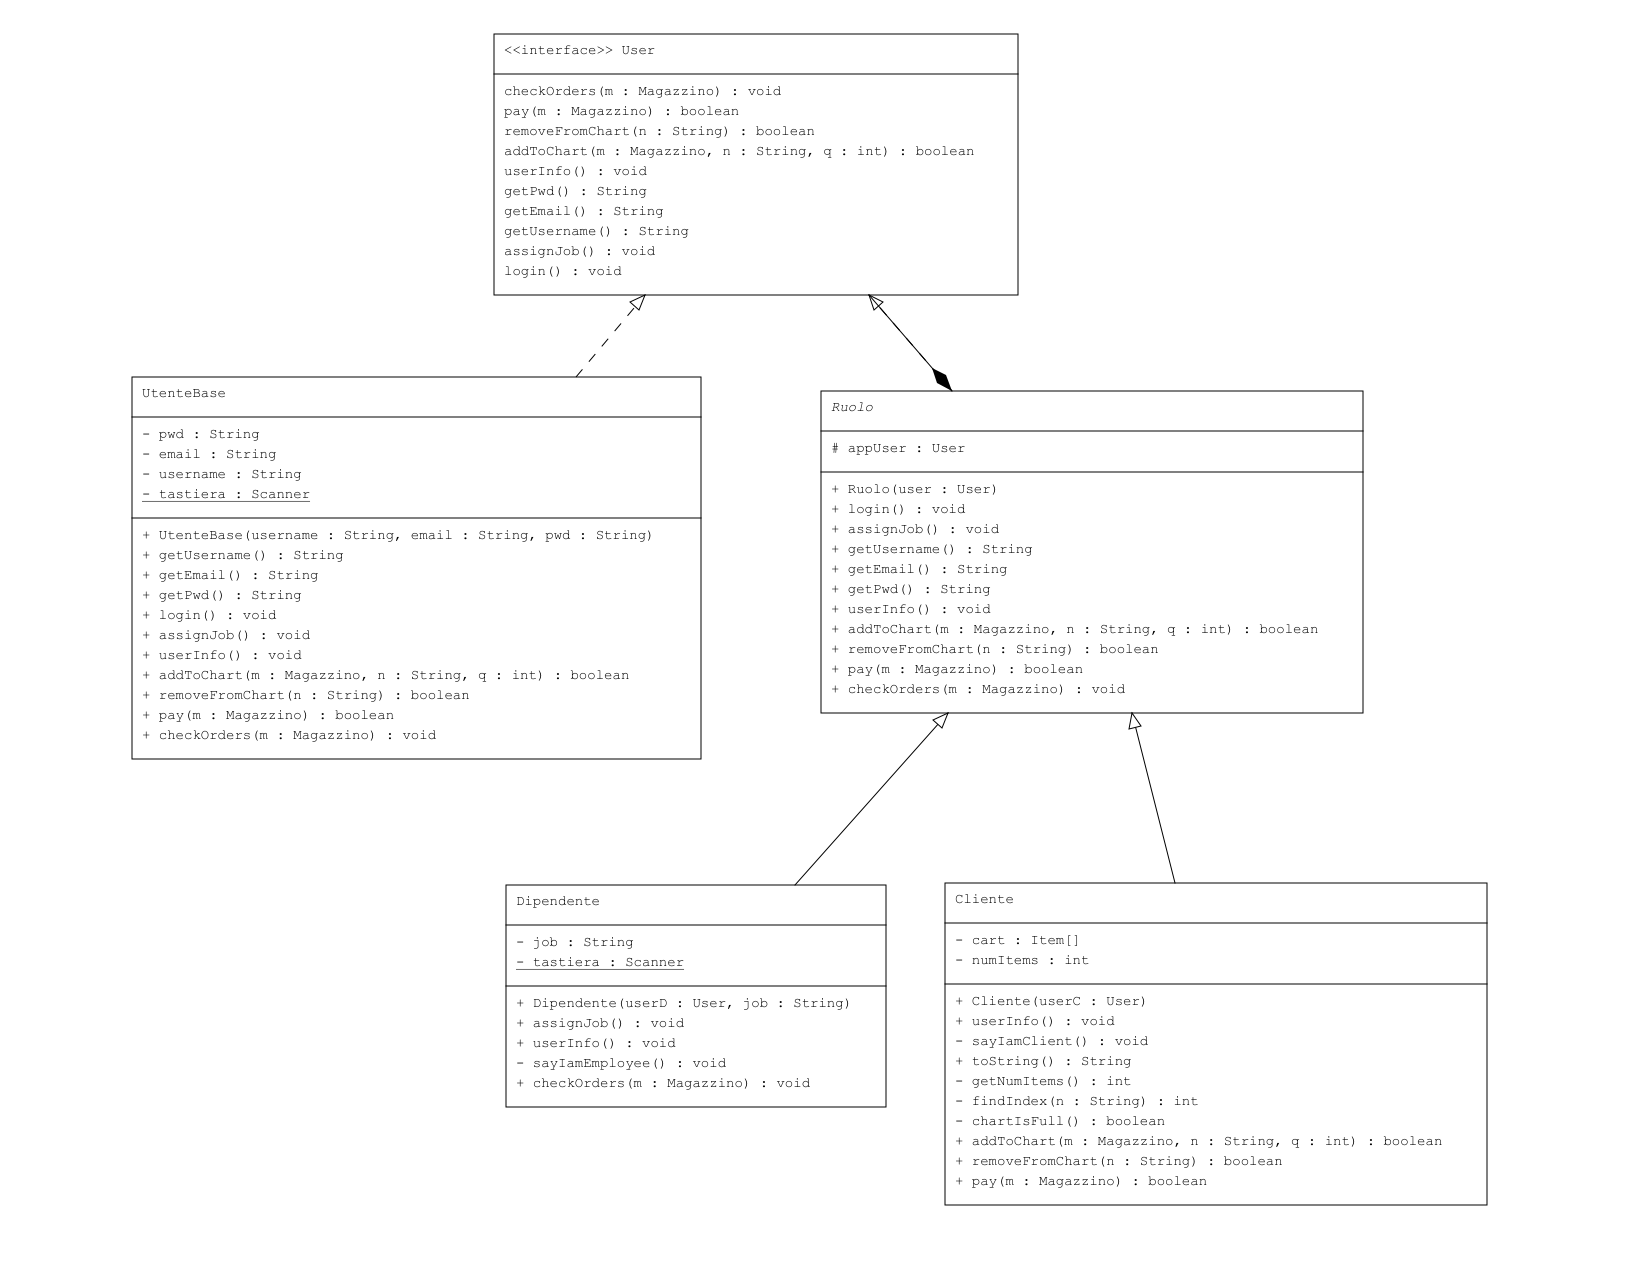
\includegraphics[width=1.4\linewidth]{images/uml_decorator.png}}
  \caption{\small Rappresentazione in UML (Unified Modeling Language) del pattern Decorator impiegato per modellare la figure del dipendente-cliente \cite{uml_riferimento}.}
  \label{fig:uml_diagram_decorator}
\end{figure}

Per implementare il pattern Decorator contestualmente al caso d'uso dell'acquisto di abiti online, abbiamo bisogno delle seguenti componenti minimali (cfr.\cite{gof_sunt}, p.65):
\begin{itemize}
    \item Un {\em Component} ({\tt User}): definisce l'interfaccia per gli oggetti a cui verranno aggiunte proprietà in modo dinamico.
    \item Un {\em ConcreteComponent} ({\tt UtenteBase}): definisce l'oggetto su cui verranno dinamicamente aggiunte le proprietà.
    \item Un {\em Decorator} ({\tt Ruolo}): mantiene una referenza al {\em Component} e definisce un'interfaccia conforme a quella del {\em Component}.
    \item Uno o più {\em ConcreteDecorator} ({\tt Dipendente, Cliente}): aggiunge le responsabilità al {\em Component}.
\end{itemize}
La relazione tra le componenti del decorator implementato per l'applicazione dell'Atelier Splendor è illustrata sotto forma di UML diagram in fig. \ref{fig:uml_diagram_decorator}.

\newpage
\lstinputlisting[label={list:user}, caption={\small User.java -- Component del pattern Decorator \cite{gof_sunt}.}]
{code/decorator/User.java}

Con riferimento a list. \ref{list:user} e a fig. \ref{fig:uml_diagram_decorator}, Tutti le componenti di questo pattern implementano l’interfaccia
{\tt User}, che specifica soltanto una serie di metodi pubblici.
Notare come sia importante mantenere l'interfaccia {\tt User} ({\em Component}) ``leggiera'', ossia: \textbf{il suo scopo è la definizione di un'interfaccia conforme, non deve contenere altri dati}. La definizione dei dati rappresentativi è competenza delle sottoclassi, altrimenti la complessità della classe {\em Component} rende i {\em decorators} troppo pesanti per essere applicati ricorsivamente. Inoltre, Mettere troppe funzionalità nella classe {\em Component} aumenta la possibilità che le sottoclassi {\em concrete} ``paghino'' per caratteristiche di cui non hanno un bisogno effettivo \cite{gof_riferimento}.

\lstinputlisting[label={list:utenteBase}, caption={\small UtenteBase.java -- ConcreteComponent del pattern Decorator \cite{gof_sunt}.}]
{code/decorator/UtenteBase.java}

Con riferimento a list. \ref{list:utenteBase} e a fig. \ref{fig:uml_diagram_decorator}, la classe {\tt UtenteBase} implementa l'interfaccia {\tt User}.

\lstinputlisting[label={list:ruolo}, caption={\small Ruolo.java -- Decorator del pattern Decorator \cite{gof_sunt}.}]
{code/decorator/Ruolo.java}

Con riferimento a list. \ref{list:ruolo} e a fig. \ref{fig:uml_diagram_decorator}, 
La classe astratta {\tt Ruolo} corrisponde al {\em Decorator} del
modello. Contiene il codice necessario per immagazzinare al suo interno
l’oggetto decorato {\tt User}, e mappa verso di lui le operazioni richieste. Si noti che questa classe implementa l’interfaccia {\tt User}, e al suo interno utilizza questa stessa interfaccia per comunicare col {\em Component} \cite{gof_sunt}.

Notare l'importanza della conformità delle interfacce: l'interfaccia di un oggetto decorato deve essere conforme all'interfaccia del {\em Component} che decora. Di conseguenza, la classe {\em ConcreteDecorator} deve ereditare da una classe comune \cite{gof_riferimento}.

Nella classe {\tt Ruolo}, notare come il \textbf{Binding Dinamico} che si ottiene ridefinendo i metodi applicati all'oggetto {\tt appUser} sia la chiave per il funzionamento corretto del pattern Decorator.

\lstinputlisting[label={list:dipendente}, caption={\small Dipendente.java -- Primo ConcreteDecorator del pattern Decorator \cite{gof_sunt}.}]
{code/decorator/Dipendente.java}

Con riferimento a list. \ref{list:dipendente} e a fig. \ref{fig:uml_diagram_decorator},
Le responsabilità specifiche riguardo la figura dell'utente dipendente
sono codificate nella classe {\tt Dipendente} \cite{gof_riferimento}. Questa classe estende le funzioni del {\em Decorator}, particolarmente aggiungendo la possibilità di controllare gli ordini presenti nel magazzino tramite il metodo {\tt checkOrders}.

\lstinputlisting[label={list:cliente}, caption={\small Cliente.java -- Secondo ConcreteDecorator del pattern Decorator \cite{gof_sunt}.}]
{code/decorator/Cliente.java}

Con riferimento a list. \ref{list:cliente} e a fig. \ref{fig:uml_diagram_decorator}, la classe {\tt Cliente} codifica la figure dell'utente cliente, dando la possibilit\'a all'utente cliente di aggiungere vestiti al carrello ({\tt  addToChart}), di rimuoverne ({\tt removeFromChart}) e di pagare effettuando l'ordine ({\tt pay}).
\\
\\
Si noti che i {\em ConcreteDecorators} definiti in questo microprototipo:
\begin{itemize}
    \item estendono operazioni esistenti del {\em Component} ({\em e.g.} il metodo {\tt  userInfo}),
    \item estendono lo stato del Component ({\em e.g.} i campi {\tt numItem}, {\tt numItems}),
    \item definiscono nuove operazioni non condivise tra i {\em ConcreteDecorators} ({\em e.g.} i metodi {\tt addToChart}, {\tt removeFromChart}, {\tt checkOrders})
\end{itemize}


\subsubsection{Comparativa Decorator vs Strategy}
Il pattern Decorator e il pattern Strategy costuiscono due modi alternativi per cambiare il comportamento di un oggetto.


\textbf{Cambiare la pelle di un oggetto, non le viscere.} Possiamo pensare al {\em Decorator} come a una pelle che ricopre l'oggetto e che ne cambia il comportamento. Se desideriamo un cambiamento più viscerale, la scelta giusta è il \textbf{pattern Strategy}.
\\
\\
Rispetto al Decorator, il pattern Strategy è la scelta giusta quando la classe {\em Component} è contenutisticamente ``pesante'' (vedi commetti sopra), e quindi rende il pattern Decorator troppo costoso da applicare.
Nel patter Strategy il {\em component} passa alcune delle sue caratteristiche a un oggetto {\em Strategy} separato \cite{gof_sunt}.
La differenza principale rispetto il decorator è che ci permette di alterare/estendere le responsabilità andando a sostituire l'oggetto {\em strategy} (cfr.\cite{gof_riferimento}, p.201).
Proseguire con riferimento al libro.


\subsection{Pattern Strategy}

Il {\em pattern Strategy} serve a definire una famiglia di algoritmi simili tra loro e dunque \textbf{intercambiabili}. In particolare, è tipica della situazione in cui vogliamo isolare l’algoritmo che svolge un certo compito, per farlo variare in modo indipendente dal resto dell’implementazione della classe.

Questo pattern suggerisce l’incapsulamento della logica di ogni
particolare algoritmo, in apposite classi, dette {\em ConcreteStrategy}, le quali implementano l’interfaccia che consente agli oggetti di interagire con loro. Questa interfaccia deve fornire un accesso efficiente ai dati del Context, richiesti da ogni ConcreteStrategy, e viceversa \cite{gof_sunt}.



\subsection{Pattern Composite}
Questo pattern ci consente di costruire una gerarchie di oggetti composti. Gli oggetti composti possono essere formati da oggetti singoli, oppure da altri oggetti composti. è utile nei casi in cui si vuole rappresentare gerarchie di oggetti tutto-parte, essere in grado di ignorare le differenze tra oggetti singoli e oggetti composti. Il fatto che l'Atelier Splendor mostra il desiderio di vendere articoli di altri brand abbiamo visto molto opportuno proporre il composite perch\'e nell'architectura potr\'a aggiungere gli articoli suoi e altri brand in modo facile e molto separato.
Il pattern viene usato nel nostro caso perché si può rappresentare il nostro magazzino come segue:

\begin{figure}[!h]
    \centering
    \makebox[\textwidth][c]{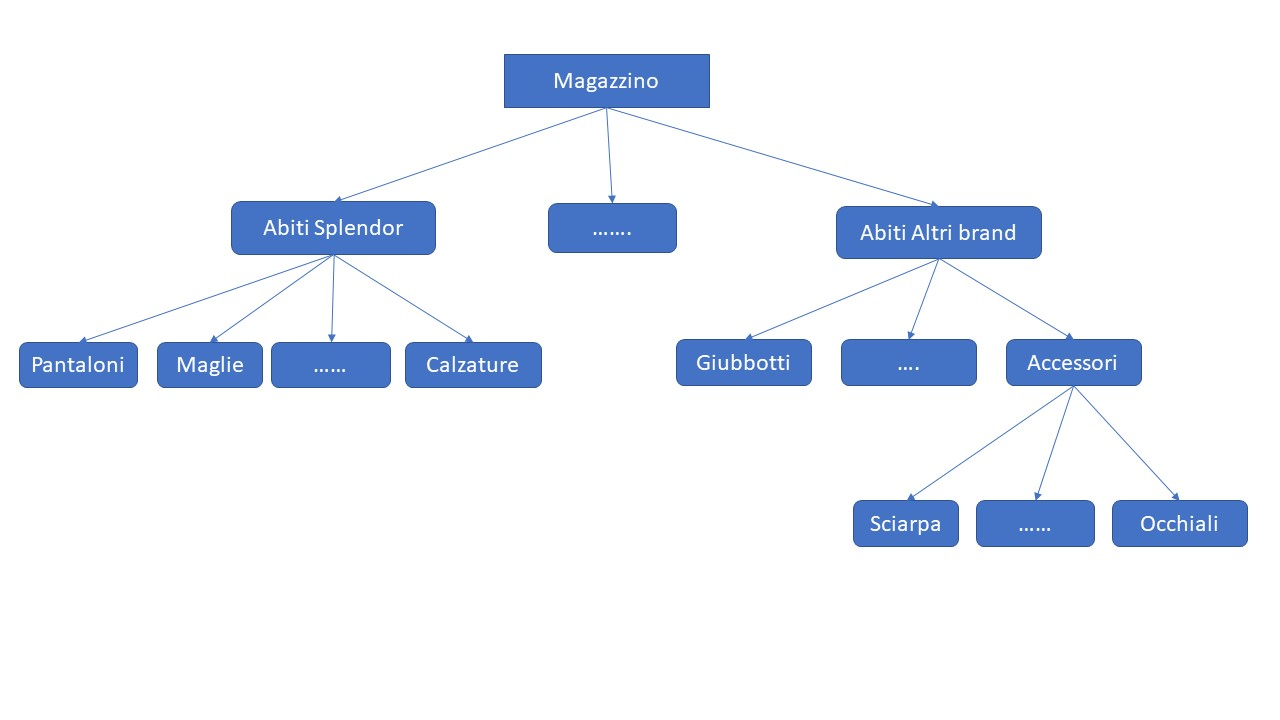
\includegraphics[width=1.1\linewidth]{images/Composite.jpg}}
  \caption{\small ...}
  \label{fig:diagram_composite}
\end{figure}

Per implementare il pattern abbiamo bisogno di :
\begin{itemize}
	\item Un \textit{Item} (è una classe astratta che fornisce le operazione base del nostro magazzino/articolo)
	\item Un \textit{CompoundItem} (La classe estende Item e si comporta sia come una parte del magazzino o come il magazzino intero a secondo di come è usato)
	\item Un \textit{SaleableItem} (Questa classe è l'articolo proprio, estende Item e ha un costruttore piu completo di CompoundItem anh )
	\item Un  \textit{SaleableItemException} (Per gestire un' \textit{exception} quando l'utente prova ad aggiungere in un \textit{SaleableItem} un \textit{Item})
\end{itemize}
\begin{lstlisting}
// The Item abstract class 
public abstract class Item {
	protected String name;

	public Item(String name) {
		this.name = name;
	}

	public abstract void describe();

	public void addItem(Item c) throws SaleableItemException {
		if (this instanceof SaleableItem)
			throw new SaleableItemException();
	}

	public void removeItem(Item c) throws SaleableItemException {
		if (this instanceof SaleableItem)
			throw new SaleableItemException();
	}

	public Item getItem(int n) {
		return null;
	}
}

//CompoundItem class
public class CompoundItem extends Item {
	private ArrayList<Item> items;

	public CompoundItem(String name) {
		super(name);
		items = new ArrayList<Item>();
	}

	@Override
	public void describe() {
		System.out.println(name);
		System.out.println("\tComposed by:");
		System.out.println("\t\t{");
		items.forEach(Item::describe);
		System.out.println("}");
	}

	public void addItem(Item c) throws SaleableItemException {
		items.add(c);
	}

	public void removeItem(Item c) throws SaleableItemException {
		items.remove(c);
	}

	public Item getItem(int n) {
		if (n<0 || n>items.size()) return null;
		return (Item) items.get(n);
	}
}

// SaleableItem class
public class SaleableItem extends Item{
	private double weight;
	private String type;
	private double price;
	private String size;
	
	public SaleableItem(String name,String type, double weight, double price,String size) {
		super(name);
		this.weight = weight;
		this.price = price;
		this.type = type;
		this.size = size;
	}

	@Override
	public void describe() {
		 System.out.println( "SaleableItem: " + name  +", type: "+type +", weight: "+weight +"kg"+", price: "+price +"€" +", size:" + size); 
		
	}
 }

 // SaleableItemException class
 public class SaleableItemException extends Exception {
	public SaleableItemException() {
		super("Not supported method, you cant add Item on SaleableItem");
	}
}
\end{lstlisting}
Come detto prima, la classe \textit{CompoundItem} può rappresentare l'intero magazzino o semplicemente una parte (categoria) di alcuni articoli. La classe \textit{CompoundItem} è usata per rapprensentare tutti gli articoli di Splenldor e quelli di altri brand che il loro insieme forma tutto il magazzino che è sempre rapprensatato da la classe \textit{CompoundItem}.
\\
La classe \textit{SaleableItem} rappresenta l'articolo venduto con tutto le caratterische possibile, ogni volta che si vuole aggiungere un articolo (\textit{SaleableItem}) si chiama la \textit{addItem} sul Magazzino (\textit{CompoundItem})
\\
\textbf{NB}: Chiamando la addItem o removeItem su \textit{SaleableItem} lancierà la \textit{SaleableItemException}


\subsection{Pattern Observer}

Il pattern \textit{Observer} (noto anche come \textit{Publish-Subscribe}) \'e un pattern TIPOPATTERNEDEFINIZIONE, che "\textit{definisce una relazione uno-a-molti tra oggetti, in modo tale che, quando un oggetto cambia stato, tutti i suoi dipendenti siano notificati e aggiornati automaticamente}" (\cite{gof_riferimento}, p.326). 
\\
\\
L'adozione di questo pattern trova le sue radici nella necessit\'a di trovare una \textit{consistenza} tra oggetti appartenenti a classi che \textit{cooperano} tra loro; una soluzione che sarebbe possibile adottare sarebbe quella di rendere queste classi strettamente dipendenti le une dalle altre, ma questo ridurrebbe la loro riusabilit\'a. La \textit{Gang of Four} cita come esempio la situazione in cui una diversa rappresentazione grafica (un grafico a barre, un grafico a torta e una rappresentazione tabellare) prendano le informazioni circa i dati da rappresentare dal medesimo \textit{data object}. Queste rappresentazioni grafiche non comunicano direttamente tra loro, ma devono comportarsi come se lo potessero fare. Quindi, nel momento in cui l'utente cambia i dati, questo cambiamento deve riflettersi in tutte le rappresentazioni grafiche di cui sopra. (cfr. \cite{gof_riferimento}, p.327)
\\
\\
Questo comportamento implica quindi, accettando il fatto di non voler creare dipendenze tra questi tre oggetti, che essi vengano notificati e coerentemente aggiornati rispetto a modifiche ed aggiornamenti che si verificano per il \textit{data object} soggiacente che li popola. Il pattern Observer viene incontro a questa esigenza. 
\\
\\
Nel nostro caso specifico, essendoci immaginati, oltre allo store on-line per la vendita dei nostri prodotti, anche l'allestimento di PopUp-Store temporanei in diverse citt\'a, l'idea che gli utenti iscritti al nostro sito per effettuare acquisti potessero essere interessati ad aggiornamenti relativi alla nostra presenza fisica sul territorio, per poter toccare direttamente con mano i capi che forniamo loro, ha portato alla presa di coscienza della necessit\'a di allestire una \textit{newsletter} che li potesse aggiornare in tal senso. Essi saranno aggiornati rispetto ad informazioni chiave quali la citt\'a ed il negozio entro cui il PopUp-Store verr\'a allestito, nonch\'e gli orari. 
\\
\\
Procediamo ora con il commento del codice utilizzato. \\
L'implementazione prevede la creazione di:
\begin{itemize}
	\item Un \textit{subject} (fornisce un'interfaccia che permette di aggiungere, rimuovere e notificare gli osservatori)
	\item Un \textit{concreteSubject} (notifica gli osservatori circa i cambiamenti del proprio stato e modifica quest'ultimo all'occorrenza)
	\item Un (...n) \textit{observer} (fornisce un'interfaccia per aggiornare gli osservatori rispetto ai cambi di stato del soggetto)
	\item Un (...n) \textit{concreteObserver} (viene informato dei cambi di stato avvenuti sul concreteSubject e usa le informazioni ottenute per aggiornarsi appropriatamente rispetto ad esso)
\end{itemize}

\begin{lstlisting}
// The Subject interface 
interface Subject {
    void registerObserver(Observer o); 
    void removeObserver(Observer o); 
    void notifyObservers();
}

// The Observer interface 
interface Observer {
    void update(String location, String store, Date openingdate, Date closingdate, float openingtime, float closingtime); 
}
\end{lstlisting}

Come abbiamo detto precedentemente, queste due interfacce permettono, rispettivamente:
\begin{itemize}
	\item SI:
		\begin{itemize}
		\item aggiungere un osservatore 
		\item rimuovere un osservatore 
		\item notificare agli osservatori i cambi di stato
		\end{itemize}
	\item OI:
		\begin{itemize}
		\item essere aggiornati rispetto ai cambi di stato del soggetto
		\end{itemize}
\end{itemize}

Ribadiamo che abbiamo definito i seguenti cambi rispetto ai quali i clienti dovranno essere aggiornati:
\begin{itemize}
	\item citt\'a entro cui si svolger\'a il PopUp-Store 
	\item il negozio che lo ospiter\'a
	\item la data di apertura e quella di chiusura
	\item l'orario entro cui esso si potr\'a trovare all'interno del negozio sopracitato
\end{itemize}

Possiamo ora passare al \textit{ConcreteSubject} e al \textit{ConcreteObserver}:

\begin{lstlisting}

// The PopUpStore class is the ConcreteSubject 
class PopUpStore implements Subject {

    private List<Observer> observers; 
    private String location;
    private String store;
    private Date openingdate;
    private Date closingdate;
    private float openingtime;
    private float closingtime;

    public PopUpStore() {
    observers = new ArrayList<Observer>();
    }

    public void registerObserver(Observer o) { 
        observers.add(o);
    }

    public void removeObserver(Observer o) { 
        int i = observers.indexOf(o);
        if (i >= 0) {
            observers.remove(i); 
        }
    }

    public void notifyObservers() {
        for (Observer observer : observers) {
            observer.update(location, store, openingdate, closingdate, openingtime, closingtime); 
        }
    }

    public void measurementsChanged() { 
        notifyObservers();
    }

    public void setMeasurements(String location, String store, Date openingdate, Date closingdate, float openingtime, float closingtime) { 
        this.location = location;
        this.store = store;
        this.openingdate = openingdate;
        this.closingdate = closingdate;
        this.openingtime = openingtime;
        this.closingtime = closingtime;
        measurementsChanged(); 
    }
}


// The ConcreteObserver class
class CurrentConditionsDisplay implements Observer, DisplayElement {
    private float temperature; 
    private float humidity; 
    private Subject PopUpStore;
    
    public CurrentConditionsDisplay(Subject PopUpStore) { 
        this.PopUpStore = PopUpStore; 
        PopUpStore.registerObserver(this);
    }
    
    public void update(String location, String store, Date openingdate, Date closingdate, float openingtime, float closingtime) { 
        this.location = location;
        this.store = store;
        this.openingdate = openingdate;
        this.closingdate = closingdate;
        this.openingtime = openingtime;
        this.closingtime = closingtime;
        display();
    }
    public void display() {
    System.out.println("We look forward to seeing you at our new Pop-Up store in " + location + ", kindly hosted by  " + store + 
    ", on the following dates: " + openingdate + " - " + closingdate + ", at the following times:" + openingtime + " - " + closingtime);
    } 
}

\end{lstlisting}

Commentando questa parte di codice, notiamo che il \textit{ConcreteSubject} \'e rappresentato dal PopUp-Store che, come anticipato, pu\'o aggiungere, rimuovere e notificare gli \textit{Observers}, andando ad aggiornare i dati relativi ai campi che definiscono il nostro PopUp-Store (tramite la comunicazione diretta con l'interfaccia \textit{Observer}). Vi \'e poi un metodo per settare questi dati. 
\\
\\
Passando invece al \textit{ConcreteObserver}, vediamo che esso ha modo di registrarsi al \textit{Subject} di nostro interesse, di aggiornare le informazioni a sua disposizione relativamente ai campi che definiscono il PopUp-Store, nonch\'e averle a disposizione tramite il suo metodo \textit{display}. 
\\
\\
Il resto del codice \'e disponibile in appendice.


\newpage

%Prints the bibliography
\printbibliography


\end{document}